\documentclass[12pt]{report}
\usepackage{arxiv}
\usepackage[utf8]{inputenc} % allow utf-8 input
\usepackage[T1]{fontenc} % use 8-bit T1 fonts
\usepackage{fancyref} % \fref \Fref
\usepackage{hyperref} % hyperlinks
\usepackage{url} % simple URL typesetting
\usepackage{booktabs} % professional-quality tables
\usepackage{amsfonts} % blackboard math symbols
\usepackage{mathtools}
\usepackage{nicefrac} % compact symbols for 1/2, etc.
\usepackage{microtype} % microtypography
\usepackage{lipsum}
\usepackage{amsmath}
\usepackage{minted}
\usepackage{amssymb}
\usepackage{xcolor} % for marking points of confusion
\usepackage{graphicx}
\usepackage{natbib}
\usepackage{caption}
\usepackage{subcaption}


\renewcommand{\fancyrefdefaultformat}{plain}
%\newcommand(\fref)[1]{\cref{#1}} % Because I started with fancyref
\newcommand{\pref}[1]{(\fref{#1})}
\newcommand{\sref}[1]{(see
\fref{#1})}

\newcommand\tab[1][1cm]{\hspace*{#1}}

\newcommand{\mc}[1]{\mathcal{#1}}
\newcommand{\bolds}[1]{\boldsymbol{#1}}

%1 Exectation value
\newcommand{\expect}[1]{\langle{}{#1}\rangle{}}

% Collections of samples
\newcommand{\mcH}{\mathcal{H}}
\newcommand{\mcE}{\mathcal{E}}
\newcommand{\mcB}{\mathcal{B}}
\newcommand{\mcV}{\mathcal{V}}
\newcommand{\mcX}{\mathcal{X}}
\newcommand{\mcY}{\mathcal{Y}}
\newcommand{\mcC}{\mathcal{C}}
\newcommand{\mcS}{\mathcal{S}}
\newcommand{\mcL}{\mathcal{L}}
\newcommand{\mcR}{\mathcal{R}}


% Microstates (bold lowercase)
\newcommand{\bh}{\bolds{h}}
\newcommand{\be}{\bolds{e}}
\newcommand{\bb}{\bolds{b}}
\newcommand{\bv}{\bolds{v}}
\newcommand{\bx}{\bolds{x}}
\newcommand{\by}{\bolds{y}}
\newcommand{\bs}{\bolds{s}}
\newcommand{\bo}{\bolds{o}}
\newcommand{\br}{\bolds{r}}

% Microstates (bold lowercase)
\newcommand{\bH}{\bolds{H}}
\newcommand{\bE}{\bolds{E}}
\newcommand{\bB}{\bolds{B}}
\newcommand{\bV}{\bolds{V}}
\newcommand{\bX}{\bolds{X}}
\newcommand{\bY}{\bolds{Y}}
\newcommand{\bS}{\bolds{S}}
\newcommand{\bT}{\bolds{T}}

% microstates explicit (bold lowercase)
\newcommand{\seth}{\{h_j\}}
\newcommand{\sete}{\{e\}}
\newcommand{\setb}{\{b\}}
\newcommand{\setv}{\{v_i\}}
\newcommand{\setx}{\{x_i\}}
\newcommand{\sety}{\{y_j\}}
\newcommand{\sets}{\{s_i\}}
\newcommand{\setr}{\{r_j\}}

\DeclareMathOperator*{\argmin}{argmin}
\DeclareMathOperator{\sgn}{sgn}

% Greek letters
\renewcommand{\l}{\lambda}
\renewcommand{\b}{\beta}
\renewcommand{\L}{\Lambda}
\renewcommand{\k}{\kappa}
\newcommand{\T}{\Theta}
\renewcommand{\P}{\Psi}
\newcommand{\coloneq}{\mathrel{\resizebox{\widthof{$\mathord{=}$}}{\height}{ $\!\!=\!\!\resizebox{1.2\width}{0.8\height}{\raisebox{0.23ex}{$\mathop{:}$}}\!\!$ }}}
\newcommand{\eqcolon}{\mathrel{\resizebox{\widthof{$\mathord{=}$}}{\height}{ $\!\!\resizebox{1.2\width}{0.8\height}{\raisebox{0.23ex}{$\mathop{:}$}}\!\!=\!\!$ }}}


\title{Anubis Learning Management System}
\date{2021-07-03}
\author{%
    John McCann Cunniff Jr \\
    New York University\\
    Brooklyn, New York \\
    \texttt{john@osiris.cyber.nyu.edu} \\
    \thanks{A special thanks to Professor Gustavo Sandoval who always believed in me} \\
}


\begin{document}

%  Title
    \begin{titlepage}

        \maketitle

        \vspace{0.3cm}
        \begin{center}
            
\includegraphics[width=0.3\textwidth]{figures/anubis-icon-1}
        \end{center}
        \vspace{0.3cm}

%  Abstract
        \begin{abstract}
            The Anubis Learning Management System (LMS) is a tool designed specifically to automate Computer Science courses. 
            Cloud IDEs integrated into Anubis provide students with a one click stable, consistent and inulated linux environment
            in their browser.
            While students work on their assignments, the provides live autograded feedback \textit{before the deadline}.
            Powerful behavioral insights are generated for TAs and Professors from data collected by the platform.
        \end{abstract}

%  Keywords
        \keywords{LMS, Cloud IDEs, Autograding, Distributed Computing, Kubernetes}

    \end{titlepage}

%  Contents
    \tableofcontents

    \pagebreak

    \begin{figure}[h]
        \centering
        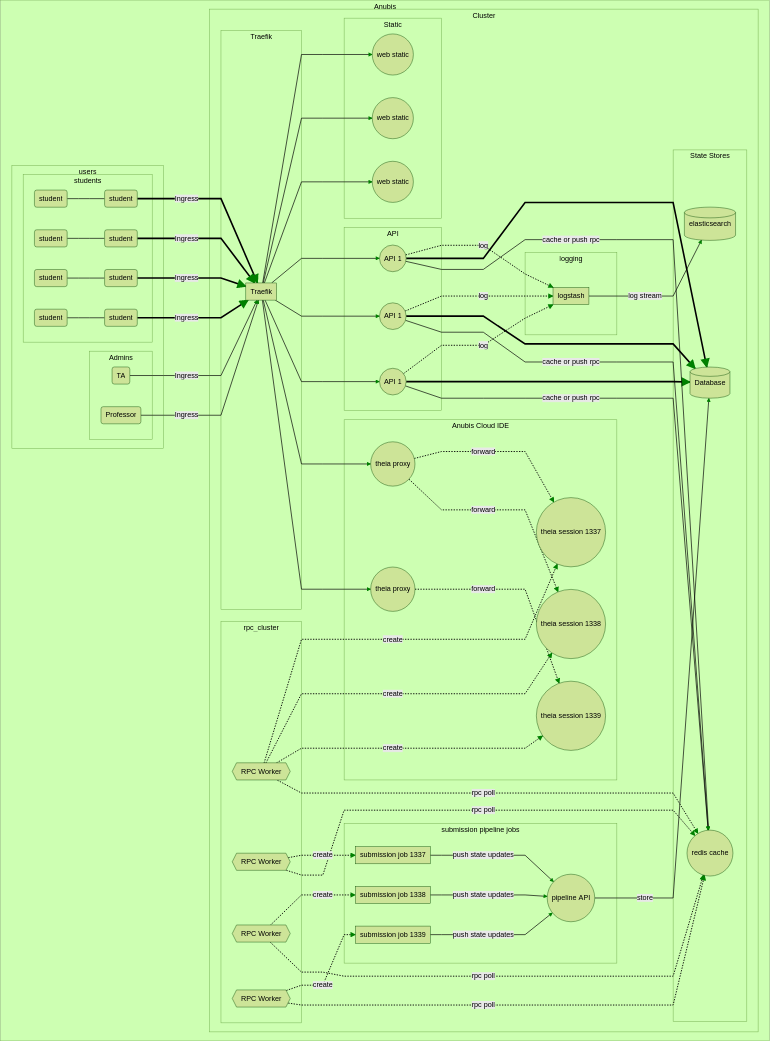
\includegraphics[width=1\textwidth]{figures/cluster.mmd}
        \caption{The Anubis Cluster\label{fig:cluster}}
    \end{figure}


%    1. overview
    \chapter{Project Overview}\label{ch:overview}

The Anubis LMS is a tool to give students live feedback on homework
assignments while they are working on them and before the deadline.
Instead of having students submit a patch file or individual files, each student
will have their own private github repository for every assignment.
The way students then submit their work is simply by pushing to their repo before
the deadline.
Students submit as many times as they would like before the deadline.

\section{Autograding}\label{sec:autograding}

When a student pushes to their assignment repo, a job is launched in the
Anubis cluster. That job will build their code, and run tests on the results.
Students can then use the live feedback to see which areas they need to improve on
before they get their final grades.


\section{Anubis Cloud IDEs}\label{sec:anubis-cloud-ides}

New in version v2.2.0, there is now the Anubis Cloud IDE. Using some kubernetes magic, we are able to
host \href{https://theia-ide.org/}{theia} servers for individual students. These are essentially VSCode instances
that students can access in the browser. What makes these so powerful is that students can access a terminal
and type commands right into a bash shell which will be run in the remote container. With this setup students
have access to a fully insulated and prebuilt linux environment at a click of a button.


\section{Insights}\label{sec:insights}

Anubis passively captures very interesting usage data from users.
Most users elect to using the Cloud IDEs as they offer an easily accessable environment.
When they do this, an autosave process pushes their work to github every few minutes,
triggering submission tests.
With this feedback loop, Anubis can capture near minute by minute progress on an assignment
for most all users.


%    2. autograding
    \chapter{Autograding}\label{ch:assignments}


\section{Assignment Structure}\label{sec:assignment-structure}

Under Anubis each student gets their own github repo for each assignment.
When they push to their repos, Anubis sees the push and runs tests on their code.
The results are then available to students on the Anubis website before the deadline.
Under this model students can push as many times as they would like before the assignment deadline.

Assignment repositories are created from template repositories.
TAs or professors can set up a repo with the necessary files or starter code for students
to work on.
Template repositories can be set up in such a way that constrains student code.
With c or c++ assignments, starter files c or c++ with a Makefile constrains students
to all start from the same point.
Instead of getting N submissions all with different file names and run options,
everyone's code will compile and run with the same commands.
This structure makes automating tests possible.


\section{Creating Autograde Tests}\label{sec:creating-autograde-tests}

Using the anubis cli, you can initialize a new assignment using
\mint{shell}|anubis assignment init <name of assignment>|

The first file you will want to edit is the \textit{meta.yml} that gets created.
This is where things like the assignment name, and due dates should be defined.
There is also a generated unique code that anubis uses to identify this assignment.
Hold on to this, as we will use it in the next step.

\begin{minted}{yaml}
assignment:
  name: "OS Final Exam"
  class: "CS-UY 3224"
  hidden: false

  # Optionally specify the github classroom link
  # for students to get their repo.
  #
  #  !! Remember to set the Custom repository
  #  !! prefix to {name}-{unique_code}
  #  !! when creating the assignment on
  #  !! Github Classroom
  github_classroom_url: "...."

  # Don't change these!
  unique_code: "839f70b2"
  pipeline_image: "registry.digitalocean.com/anubis/assignment/{unique_code}"

  # Specify the important dates here
  # * Remember! These are interpreted as America/New_York *
  date:
    release: "2021-05-17 06:00:00"
    due: "2021-05-19 06:00:00"
    grace: "2021-05-19 06:30:00"

  # This description will be shown to the user on the Anubis website.
  description: |
    Good luck.
\end{minted}

Here is an example generated meta.yml from the OS final exam this semester.
The only fields that you will need to fill in are the github classroom url.
This is the URL that is given to you when you create a github classroom assignment.
That link will then be provided as a button for students to click in the frontend.


\section{Writing Autograde Tests}\label{sec:writing-autograde-tests}

All the files to build and run a complete anubis pipeline image will be dropped into the new directory.

\begin{minted}{text}
new-assignment
|- assignment.py
|- Dockerfile
|- meta.yml
|- pipeline.py
|- test.sh
`- utils.py
\end{minted}

The only thing you will ever need to edit is assignment.py.
This is where you define your build and test code.
Just like all the other cool libraries out there, the anubis pipeline works
through hooking functions.
Here is a minimal example of an assignment.py that will build and run a single simple test.

\begin{minted}{python}
from utils import register_test, register_build, exec_as_student
from utils import (
    TestResult, BuildResult, Panic, DEBUG,
    xv6_run, did_xv6_crash,
    verify_expected, search_lines, test_lines
)

@register_build
def build(build_result: BuildResult):
    stdout, retcode = exec_as_student('make xv6.img fs.img')

    build_result.stdout = stdout.decode()
    build_result.passed = retcode == 0


@register_test('test echo')
def test_1(test_result: TestResult):
    test_result.stdout = "Testing echo 123\n"

    # Start xv6 and run command
    stdout_lines = xv6_run("echo 123", test_result)

    # Run echo 123 as student user and capture output lines
    expected_raw, _ = exec_as_student('echo 123')
    expected = expected_raw.decode().strip().split('\n')

    # Attempt to detect crash
    if did_xv6_crash(stdout_lines, test_result):
        return

    # Test to see if the expected result was found
    verify_expected(stdout_lines, expected, test_result)
\end{minted}

There are a couple functions to point out here.
The \textit{register\_build} and \textit{register\_test} decorators are how
you tell anubis about your build and test.
The \textit{exec\_as\_student} function is how you should call any and all student code.
It lowers the privileges way down so that even if the student pushes something
malicious, they are still low privileged enough where they can not do much.
It also adds timeouts to their commands.
Boxing student code in like this is absolutely essential.
Do not underestimate the creative and surprising ways students will find to break things.

Each test is passed a \textit{test\_result} object.
This object has 3 fields.
All you need to do is set the fields on the \textit{test\_result} object.
The results will then be reported to the anubis api, and then to the student.

\begin{minted}{python}
class TestResult(object):
    def __init__(self):
        # The standard out for the students tests. You can
        # add extra text in this field as needed.
        self.stdout: str = None

        # The message is an optional parameter that will
        # insert a short message in bold above the standard
        # out on the website frontend.
        self.message: str = None

        # Passed should be a boolean value. True if the test
        # passed, and False if it did not.
        self.passed: bool = None
\end{minted}

The functions \textit{run\_xv6} and \textit{did\_xv6\_crash} are very specific to the Intro to OS needs.
There are also some general functions that are just as helpful.

\begin{minted}{python}
def exec_as_student(cmd, timeout=60) -> typing.Tuple[bytes, int]:
    """
    Run a command as the student. Any and all times that student
    code is run, it should be done through this function. Any other
    way would be incredibly insecure.

    :param cmd: Command to run
    :param timeout: Timeout for command
    :return: bytes output, int return code
    """


def verify_expected(
    stdout_lines: typing.List[str],
    expected_lines: typing.List[str],
    test_result: TestResult,
    case_sensitive: bool = True,
    search: bool = False
):
    """
    Check to lists of strings for quality. Will strip off whitespace from each line
    before checking for equality. The stdout_lines should be from the student code.
    The expected_lines should then be whichever lines are expected for this test.

    * The fields on the test_result object will be set automatically based on if the
    expected output was found. *

    :param stdout_lines: students lines as a list of strings
    :param expected_lines: expected lines as a list of strings
    :param test_result: TestResult object for this test
    :param case_sensitive: boolean to indicate if the comparison should be case sensitive
    :param search: boolean to indicate if the stdout should be searched instead of
                   directly compared for equality
    :return:
    """


def test_lines(
        stdout_lines: typing.List[str],
        expected_lines: typing.List[str],
        case_sensitive: bool = True
) -> bool:
    """
    Test lines for exact equality. Whitespace will be stripped off each line automatically.

    * Optionally specify if the equality comparison should be case sensitive *

    >>> test_lines(['a', 'b', 'c'], ['a', 'b', 'c']) -> True
    >>> test_lines(['a', 'debugging', 'b', 'c'], ['a', 'b', 'c']) -> False
    >>> test_lines(['a', 'b'],      ['a', 'b', 'c']) -> False

    :param stdout_lines: students standard out lines as a list of strings
    :param expected_lines: expected lines as a list of strings
    :param case_sensitive: optional boolean to indicate if comparison should be case sensitive
    :return: True if exact match was found, False otherwise
    """


def search_lines(
        stdout_lines: typing.List[str],
        expected_lines: typing.List[str],
        case_sensitive: bool = True
) -> bool:
    """
    Search lines for expected lines. This will return true if all expected lines are in the
    student standard out lines in order. There can be interruptions in the student standard out.
    This function has the advantage of allowing students to still print out debugging lines
    while their output is still accurately checked for  the expected result.

    >>> search_lines(['a', 'b', 'c'], ['a', 'b', 'c']) -> True
    >>> search_lines(['a', 'debugging', 'b', 'c'], ['a', 'b', 'c']) -> True
    >>> search_lines(['a', 'b'],      ['a', 'b', 'c']) -> False

    * Optionally specify if the equality comparison should be case sensitive *

    :param stdout_lines:
    :param expected_lines:
    :param case_sensitive:
    :return:
    """
\end{minted}


\section{Deploying Autograde Tests}\label{sec:deploying-autograde-tests}


Once you have tests written, then it is time to push them to Anubis.
The next thing that needs to be done is push the image to the docker registry and
upload the assignment data to anubis.
This is as simple as running two commands:

\begin{minted}{shell}
# sends assignment metadata to anubis api
anubis assignment sync

# builds then pushes the assignment
# pipeline image to the registry
anubis assignment build --push
\end{minted}


\section{Submission Pipelines}\label{sec:submission-pipelines}

\begin{figure}[ht]
    \centering
    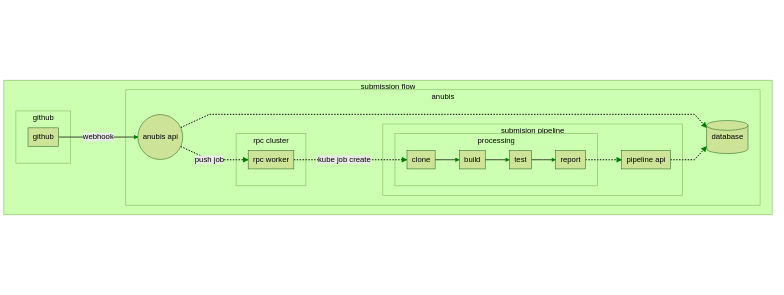
\includegraphics[width=1\textwidth]{figures/submission-flow.mmd}
    \caption{Submission Pipelines are a complex multi service data flow. \label{fig:submission-flow} }
\end{figure}

Submissions Pipelines~\fref{fig:submission-flow} are where the autographing is really happening.
When students push code to their github repositories, Anubis sees the new
commits and creates a pipeline job.
Each commit to student github repository gets a new Submission Pipeline.

\subsection{Kubernetes Job}\label{subsec:kubernetes-job}

Each Submission Pipeline is a \href{https://kubernetes.io/docs/concepts/workloads/controllers/job/}{Kubernetes Job}.
There are certain assurances that can be made when using Kubernetes Jobs.
If there is an issue on one node on the cluster that prevents a submission job from finishing,
Kubernetes will reschedule and retry the Submission Pipeline elsewhere.

\subsection{Pipeline State Reporting}\label{subsec:pipeline-state-reporting}

Some assignment tests will also take a long time to process each submission.
Due to this reality, live state updating was added to the Submission Pipelines.

There is an internal REST api that is only for submission pipelines to report state to.
This pipeline is called the \textit{pipeline-api}.
The \textit{pipeline-api} is specifically a subset of the main api.
It has different view functions defined for it.
The purpose of these special api servers is to take state updates from submission
pipelines and update the database.

If a submission is processing the website will poll for updates.
This complex multi service state reporting model is how results from isolated
submission pipelines appear on the website for students as they happen.

\subsection{Pipeline Stages}\label{subsec:pipeline-stages}

It is important to note that at each stage of the submission pipeline,
we will be moving execution back and forth between two unix users.
There will be the entrypoint program managing the container as user \textit{anubis}.
The \textit{anubis} user will have much higher privileges than the \textit{student} user.
The \textit{student} user will be used whenever executing student code.
It will not have any level of access to anything from the \textit{anubis} user.

\subsubsection{Clone}

n this initial stage, we will pull the current repo down from github.
After checking out the commit for the current submission, we will also delete
the \textit{.git} directory as it is not needed.
Lastly we will chown the entire repo as \textit{student:student}.
This will then be the only place in the container that the student user
can read or write to (other than /tmp of course).

\subsubsection{Build}

At this stage we hand execution off to student code for the first time.
Code must be built as the student user.
The function that was marked with the \textit{register\_build} decorator handles this phase.
The stdout and return code of the build will be captured by the \textit{anubis} user.
For most assignments, the success of the build is determined by the return code.
No extra parsing of the stdout should be necessary.

\subsubsection{Test}

Tests are defined on a per-assignment basis.
Again, student code will be executed for this step.
That code must be executed as the \textit{student} user.

Each test is defined as a python function that was decorated with the
\textit{register\_test} decorator.
The function should run the student code for whatever they are testing, then
confirm that the standard out matches whatever was expected.

The state updating at this step is automatic.
After each test hook is called, the results will automatically be sent off to the
\textit{pipeline-api}.

After the last test is called, the pipeline sends a special state update stating that
the submission tests have completed.
It is important that this step happens as it is where the submission is marked as
processed.

\subsection{A Word on Isolation}\label{subsec:a-word-on-isolation}


We are executing student code in the submission pipeline containers.
Due to this reality, the pipelines are designed from the ground
up to be isolated in whatever way they can be.

There is a special \href{https://kubernetes.io/docs/concepts/services-networking/network-policies/}{kubernetes network} that is applied to 
all the submission pipeline pods.
This policy limits the pod to only being able to connect to the \textit{pipeline-api}
service.
Using simple resource requests and limits in kubernets enables
limits on resources like cpu and memory.

In early versions of Anubis, there were not memory limits on submission
containers. 
Several students would push code that would blow up in memory. 
These students were not acting malicious, they just did not understand
how memory works in C that well.
When this would happen, the node would be quickly drained of available memory,
and the OOM killer would start taking other processes and containers down.
Obviously this lead to sensible resources limits being placed
on student code. In more modern versions of Anubis there are proper isolation and
resource limits that are placed on students.




%    3. cloud ides
    \chapter{Anubis Cloud IDEs}\label{ch:cloud_ides}

\begin{figure}[ht]
    \centering
    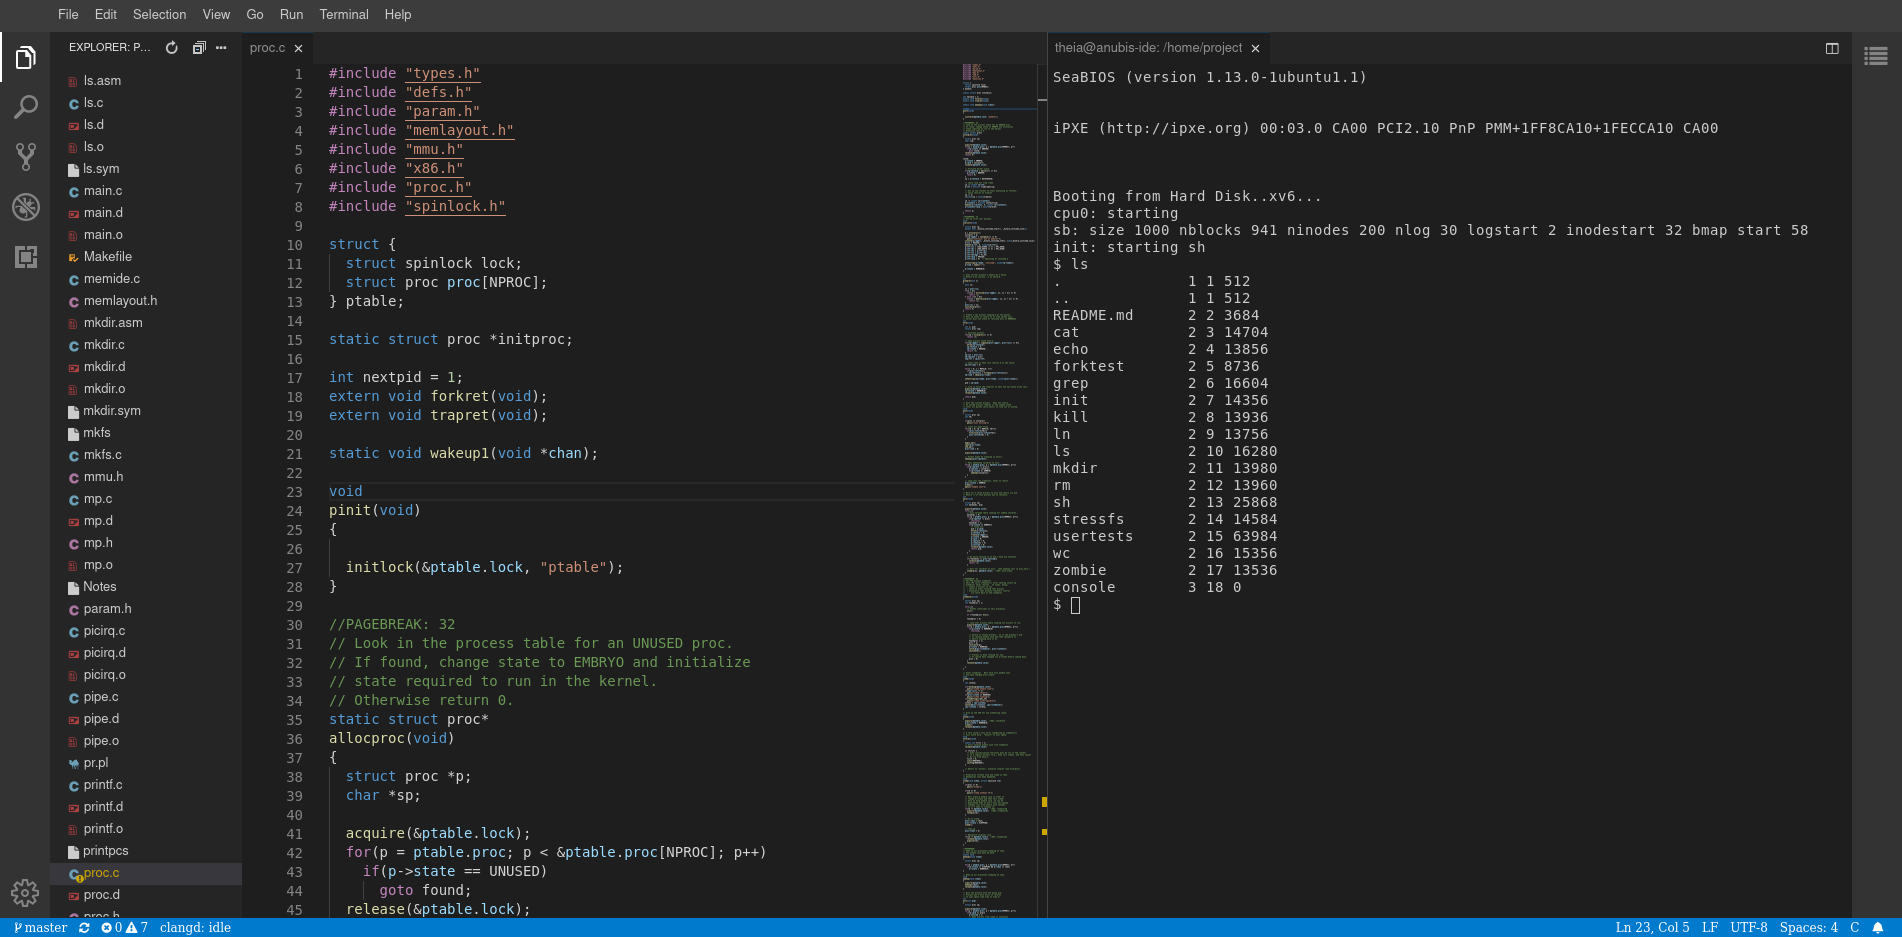
\includegraphics[width=0.9\textwidth]{figures/theia2}
    \caption{Anubis Cloud IDE\label{fig:theia2}}
\end{figure}

\section{Cloud IDE Overview}

One of the more exciting new features of Anubis is that of the Cloud IDEs.
Anubis Cloud IDEs are \href{https://theia-ide.org/}{Theia} IDE servers that run in containers.
Since the containers are themselves linux environments, we can allow students
to run commands in that environment with the built in terminal in Theia.

\section{Packaging of Course Software}

Taking these IDE container servers to the next level, we can add whatever 
other software is necessary for the course.
Packaging the tools that students need into a custom Theia server container
built specifically for the needs of the course are then available with 
one click to students.
Nothing to install, nothing to setup.
All students need is a modern web browser and an internet connection.

For many years, the CS-UY 3224 (Intro. to Operating Systems) course
jumped around from one VM solution to another.
Each one posed challenges with setting up for some subset of students.
By using the Anubis IDEs, this issue is completely removed.
The tools necessary for the homeworks are packaged into the of build 
of Theia that is used for the course.
The course VMs are then no longer necessary.
Students have access to all the tools they need through the Cloud IDE
with one click.

\section{IDE Guarentees}

Leveraging some magic that Kubernetes and containers give us,
we can provide a fully insulated linux environment for hundreds of
students concurrently.

Any solution in the cloud that we provide for student need certain assurances.
The majority of students will rely on the Cloud IDEs to do their homework.
The system cannot fail right before a deadline when the load on Anubis is greatest.
Cloud IDEs need to be scalable.
This requires the system to distribute Cloud IDE instances across multiple nodes. 
Networking traffic to Cloud IDEs need to also be automatically detected and balanced.

\subsection{Scaling IDEs}

Kubernetes tracks what resources are reserved for specific containers.
When it runs out of a resource like memory of cpu, it will automatically
add more nodes to the cluster and spread the load.
There resource reservations are added to each student Cloud IDE.
If there are more students asking for Cloud IDEs resources than exist
in the cluster, it will automatically scale to handle the load.

\subsection{Balancing Network Traffic}

There is a service in Anubis whose only purpose is to route
student requests to IDE instances. 
This service is called the \textit{theia-proxy}. 
See~\fref{fig:anubis-ide} to see where the \textit{theia-proxy}
fits into the deployment.

\begin{figure}
    \centering
    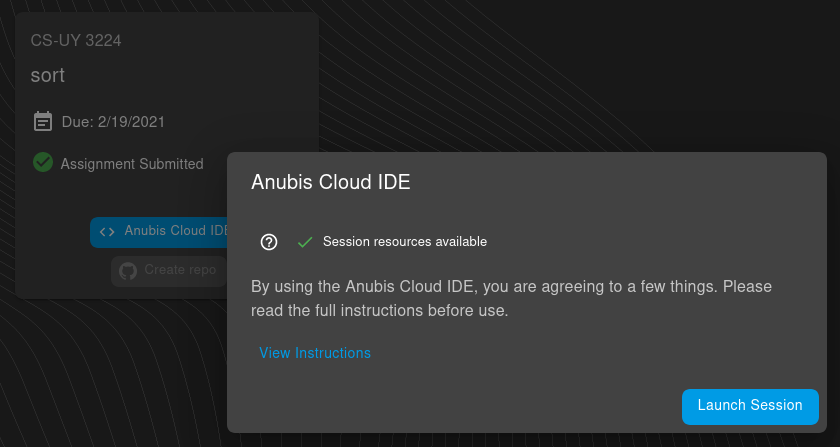
\includegraphics[width=0.5\textwidth]{figures/theia1.png}
    \caption{Launch Anubis Cloud IDE\label{fig:theia1}}
\end{figure}

When a student clicks the button to create a Cloud IDE, 
an IDE pod is created for that student~\fref{fig:theia1}.
At the time that the pod is created, the in cluster ip address
of that pod is recorded in the database (called a \textit{ClusterIP}).

Once the Cloud IDE has been initialized, then a \textit{goto ide} button
will become available.
When clicked, the student will be redirected to \textit{ide.anubis.osiris.services}.
That domain points to the \textit{theia-proxy} service.
The proxy then parses the cookie set for the user, and pulls the 
cloud ide pod ip address from the database.
The proxy then forwards the request to the proper Cloud IDE container.

The \textit{theia-proxy} service is setup with a 
\href{https://kubernetes.io/docs/tasks/run-application/horizontal-pod-autoscale/}{Horizontal Pod Autoscaler} or HPA.
These are special kubernetes resources that will automatically add or subtract containers
from a deployment based on the resources in use.
The HPA for the \textit{theia-proxy} is configured to detect when 
there is prolonged cpu load and automatically add new proxy containers.
The load balancer will then automatically distribute incomming connections
between \textit{theia-proxy} containers.


\section{IDE Pod Design}

\begin{figure}[ht]
    \centering
    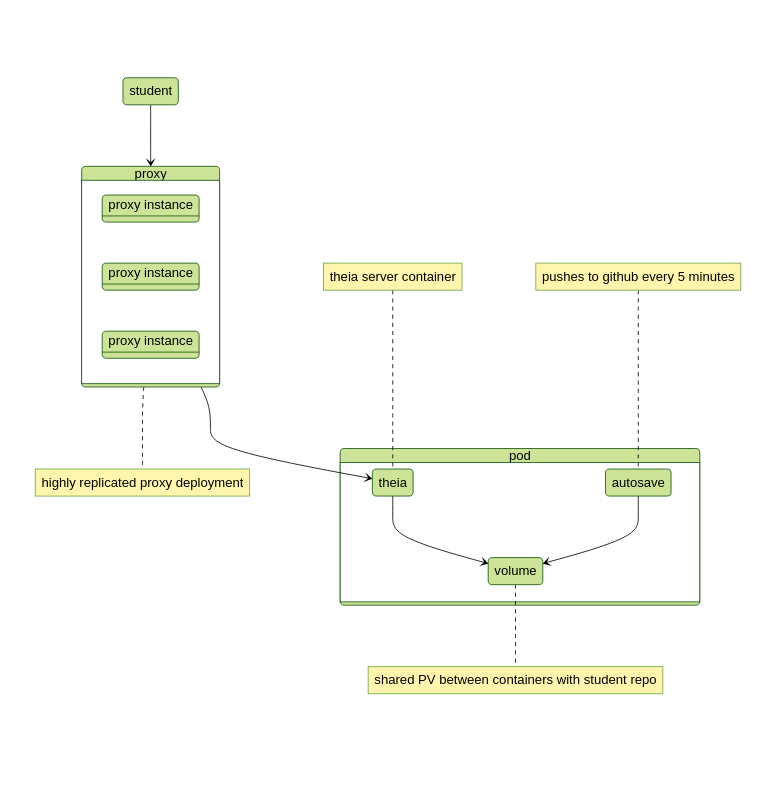
\includegraphics[width=0.5\textwidth]{figures/theia-pod.mmd}
    \caption{Anubis Cloud IDE design\label{fig:anubis-ide}}
\end{figure}

The Cloud IDE pod design requires some finesse. 
There are a couple of things about theia that make it so that
we need to do some rather fancy things in Kubernetes to make 
the setup work.

The main thing that we need to handle is the fact that theia requires a websocket connection between the browser and
theia server instance. When the pods are allocated Anubis records the ClusterIP in the database. Then when we need to
initialize a client connection Anubis uses this saved ClusterIP to forward requests (both http and websockets) to the
correct pod.

These IDE servers are temporary. When the student finishes working (or after a timeout) we reclaim the resources by
deleting the pod and shared volume. Because of this, we needed some form of autosave. Saving is pushing to github.
The issue we need to contend with is automatically committing and pushing to github without exposing a sensitive
password or api token to the users. We handle this by having a second container whose only role is committing and
pushing to github. The credentials live in that container, completely separate and inaccessible to the user who
may be working in the other theia server container. These two containers are connected by a shared volume mounted
at `/home/project` in both containers. This volume is relatively small (~50MiB).

With this setup, we have autosave running in the background while being completely hidden from the user. When
explaining autosave to students we usually just say "it is witchcraft, just trust that it works".


With these lightweight containerized theia servers, we are able to support significantly more concurrent users than
if we had elected to implement a cloud VM solution. Because Anubis Cloud IDEs do not need to virtualize hardware,
the resources on the system for each user is significantly less. Given the resources that we have on Digital Ocean,
we would be able to have maybe 20-30 concurrent users using cloud virtual machines. With our containerized theia,
we can handle all ~130 students in CS-UY 3224 at the same time with room to breath.


%    4. insights
    \chapter{Insights}\label{ch:insights}

\section{High Level Usage Stats}\label{sec:high-level-usage-stats}

There is a unavoidable wave of complains that flow in for every assignment in CS-UY 3224
in the day or so before a deadline.
The most common is the classic \textit{you did not give us enough time} excuse.
Even if the assignment was assigned weeks before the deadline.

Something unique about spring semester of 2021 for CS-UY 3224 was the introduction of the public usage graph on Anubis.
This graph~\fref{fig:public-usage} is generated every few minutes from live usage data in Anubis.
It shows the number of Cloud IDEs and submissions per hour for each assignment.
Although it also has the due date for different assignments marked, you could easily deduce the
due date for each.
It is always the day that the usage spikes from basically nothing to hundreds of submissions per hour.

Our response to students asking for extensions was often just showing the usage graphs in lecture.
These graphs are an interesting experiment in student behavior.
They can prove that the majority of students wait until the very last minute to do an assignment
regardless of how long the assignment has been released.
I think most educators have assumed this to be the case, but generating near live graphs from 
this behavior is certainly an unique feature of Anubis.  

\begin{figure}[ht]
    \centering
    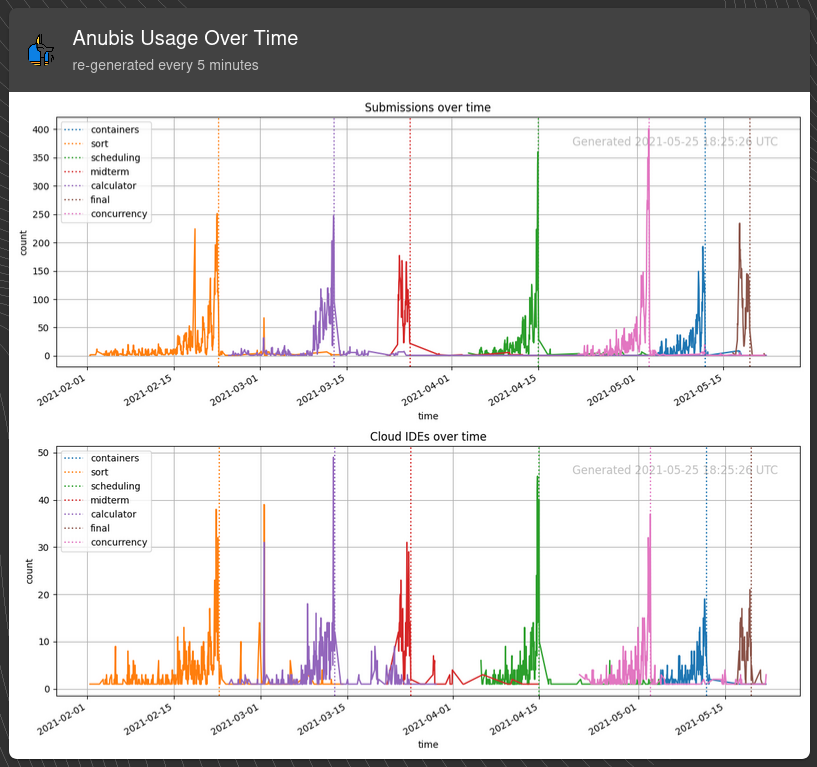
\includegraphics[width=0.5\textwidth]{figures/public-usage-1}
    \caption{Public Usage Graph\label{fig:public-usage}}
\end{figure}

\section{Class Level Autograde Results}\label{sec:class-level-results}

A special visual is generated specifically for visualizing the success of an assignment at a glance.
This visual is called the Anubis Sundial~\fref{fig:autograde-sundial-1}.
It is a radial graph that shows the proportion of students that are passing/failing tests
for a specific assignment.

\begin{figure}[ht]
    \centering
    \begin{subfigure}{0.5\textwidth}
        \centering
        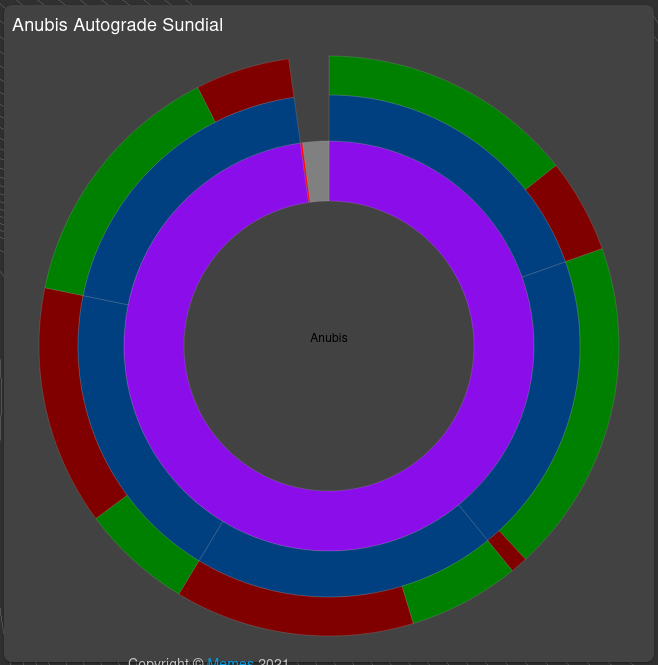
\includegraphics[width=0.9\textwidth]{figures/sundial-1}
        \caption{The Anubis Sundial.\label{fig:autograde-sundial-1} }
    \end{subfigure}%
    \begin{subfigure}{0.5\textwidth}
        \centering
        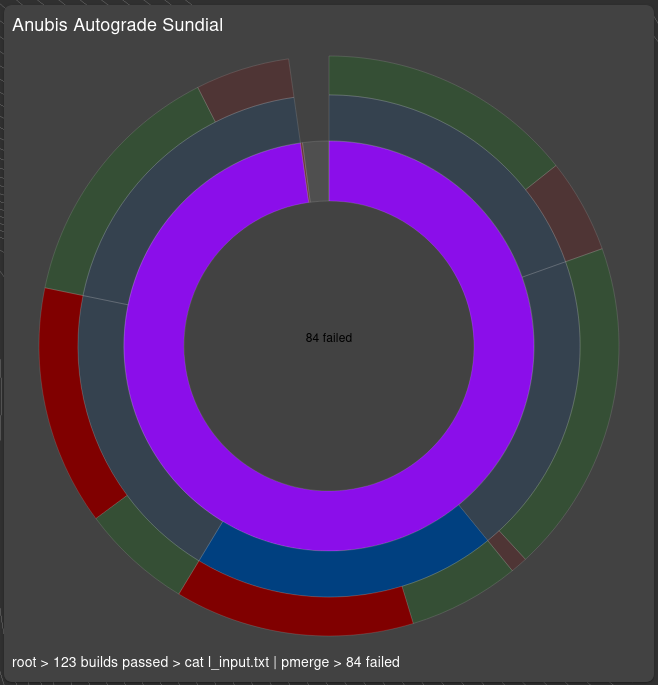
\includegraphics[width=0.9\textwidth]{figures/sundial-3}
        \caption{Many students failed the long file lines test.\label{fig:autograde-sundial-3} }
    \end{subfigure}
\end{figure}

With this simple visualization professors can see which tests students are struggling with.
Sundials are generated live.
At any time, even before the due date, they will be available.
For course administrators, this means that they can see which tests students are struggling with.


Take the simple example in~\fref{fig:autograde-sundial-3}.
By mousing over the sundial, we can see that the tests with long file lines are failing.
This information can then lead to long line buffering being covered again in lecture or
recitation.

\section{Student Level Autograde Results}\label{sec:student-level-results}

Given the structure of Anubis assignments, coupled with the Anubis Cloud IDEs we can
track and measure each student's progress through an assignment.
We can track and measure when students start and finish their assignments,
and how long it takes them to pass specific tests.
In the autograde results panel, a "visual history" is generated for each student.
It shows when students started their assignment, then for each submission if their
build passed or failed and how many tests passed.
If they used the Anubis Cloud IDEs as most students do choose to,
then the graph generated shows a near minute by minute representation of which
challenges they faced and how long it took for them to overcome them.

\begin{figure}[ht]
    \centering
    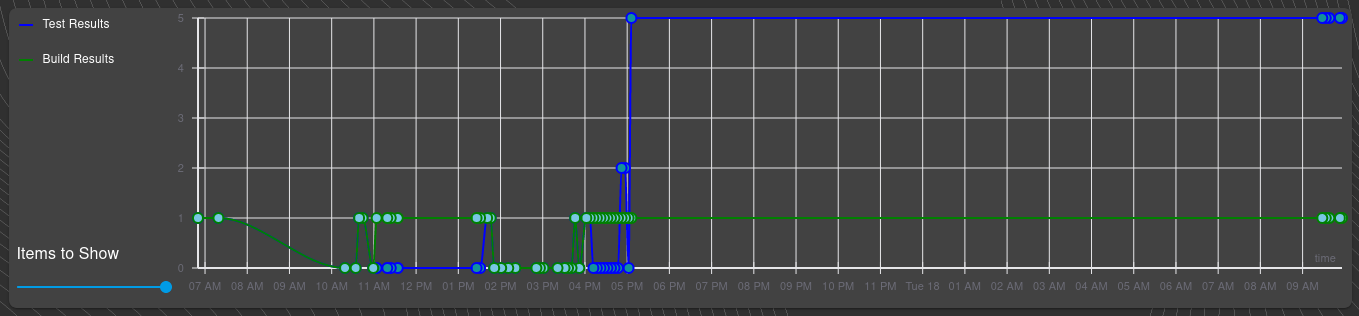
\includegraphics[width=0.9\textwidth]{figures/student-assignment-visual-history-1}
    \caption{A Student Visual History\label{fig:student-assignment-visual-history-1}}
\end{figure}

The example in~\fref{fig:student-assignment-visual-history-1} shows the build as the green
line, and the assignment tests as the blue line.
We can see that this student spent a good deal of time on the first day
just getting their tests to pass, only to revisit their work the next day probably to
clean up their submission.


%    5. services
    \chapter{Services}\label{ch:services}


\section{Traefik Edge Router}\label{sec:traefik}

\begin{figure}[ht]
    \centering
    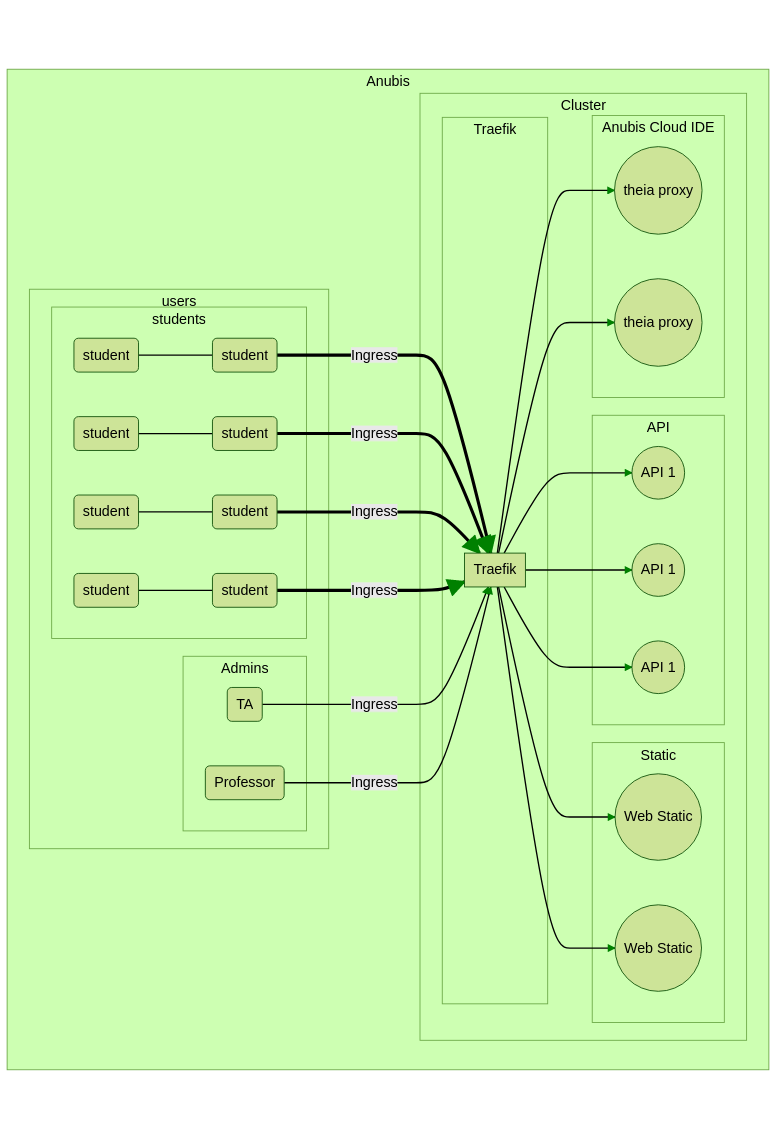
\includegraphics[width=0.5\textwidth]{figures/traefik.mmd.png}
    \caption{Traefik Traffic in Anubis\label{fig:traefik}}
\end{figure}

For our edge router, we use traefik~\ref{fig:traefik}.
Traefik will be what actually listens on the servers external ports.
All external traffic will be routed through Traefik.
Above all else, we will be using Traefik's powerful routing features to handle the ingress of requests.

Traefik lets us do some spicy and powerful stuff.
We can route requests to different services based off predefined rules,
and even change requests as they pass through.

Among other things, the routing rules make it so that we can have
both the static store and api on the same domain.
The rules are set up such that every request that
starts with a path of \textit{anubis.osiris.services/api/*} goes to the api~\ref{sec:api} service.
All other requests \textit{anubis.osiris.services/*} are routed to the web static~\ref{sec:web} service.

In addition to having the web static~\ref{sec:web} and the anubis api~\ref{sec:api} services on
the same domain, we can add routing rules for the theia-proxy~\ref{sec:theia-proxy} service.
Anything that is \textit{ide.anubis.osiris.service/*} will be routed to the theia-proxy service~\ref{sec:theia-proxy}.

By leveraging these features of Traefik, we can make it appear that
the services work different when being accessed externally.


\section{Anubis API}\label{sec:api}

The API is the backbone of Anubis.
It is where most of the heavy lifting is done.
The service relies on both the cache~\ref{sec:caching} and mariadb data
stores~\ref{sec:data-stores} to maintain state.

The Anubis API is itself nothing more than a simple \href{https://flask.palletsprojects.com/en/2.0.x/}{Flask} app.
As of version \textit{v3.1.16} it is about 25,000 lines of python.

\subsection{Zones}\label{subsec:api-zones}

The API is split into two distinct, and uniquely treated zones.
There is a public and a admin zone.
All endpoints for Anubis fall within one of these zones.
In the source code for Anubis, the views for these zones exist
in separate public and admin python modules.

All public view endpoints will start with the url \textit{anubis.osiris.services/api/public/*}.
Similarly, the admin view endpoints will start with \textit{anubis.osiris.services/api/admin/*}.

\subsection{Public Zone}\label{subsec:api-public-zone}
The majority of the public API does require authentication.
This is mostly handled by the \textit{@require\_auth} decorator applied to the view function.
Additional checks will be done to verify that the resource, or calculation being requested are
something the requester (the user making the request) is authorized to see.
The distinction must be made that public here means that it is public to users.
Students that open Anubis in a web browser and navigate through their submissions and assignments
will only be using the public API.

\subsection{Admin Zone}\label{subsec:api-admin-zone}
The admin api zone is where all the special endpoints that require higher than student level permission reside.
When a TA or Professor uses any functionality of the Admin Panel, they are using these special
admin flask views.
All of the view functions in the admin api module have decorators like \textit{@require\_admin()} or
\textit{@require\_superuser()}.
These protect the endpoints from anyone without admin permissions on at least one course.
Additional checks are then performed on each endpoint to verify that whatever resource is being requested
or modified is allowed by the current user.

\subsubsection{Course Context}\label{subsubsec:course-context}
Most view functions for the admin api require a \textit{course context} set in the cookie of the request.
When multi-course management was added to Anubis, most all the view functions for the admin api
needed to be made \textit{"course aware"}.
What that means is that there needed to be a check that the user making the request is an admin \textit{and} is
an admin for the course that that resource resides under.

\subsection{Health Checks}\label{subsec:api-health-checks}
There are very simplistic health checks in the api that make debugging issues much easier.
The endpoint \textit{anubis.osiris.services/} will run the following view function:

\begin{minted}{python}
    @app.route("/")
    def index():
        Config.query.all()
        cache_health()
        return "Healthy"
\end{minted}

The view checks that the database~\ref{subsec:mariadb} is accessible by running a query, then calls a function that relies on the
redis cache~\ref{subsec:caching}.
While this view function may be simple, it is quite effective.
Most of the incidents of degraded service or downtime come down to either the database or cache being temporary
unavailable.

\subsection{Responsibilities}\label{subsec:api-responsibilities}

The Anubis API is responsible for handling most basic
IO, and state managing that happens on the cluster.
Some of this includes:

\begin{itemize}
    \item Authenticating users
    \item Providing Class, Assignment, and Submission data to the frontend
    \item Handling github webhooks
    \item Handling reports from the submission pipeline cluster
    \item Handling regrade requests
    \item Initializing new IDE sessions
\end{itemize}

\subsection{Authentication}\label{subsec:api-authentication}

To authenticate with the api, a token is required.
The only way to get one of these tokens is through NYU Single Sign On.
By doing this, we are outsourcing our authentication.
This saves a lot of headaches while being arguably more secure than if we rolled our own.

All of this is about 20 lines on our end.
All that is necessary are some keys from NYU IT.


\section{Anubis Web Static}\label{sec:web}

\begin{figure}[ht]
    \centering
    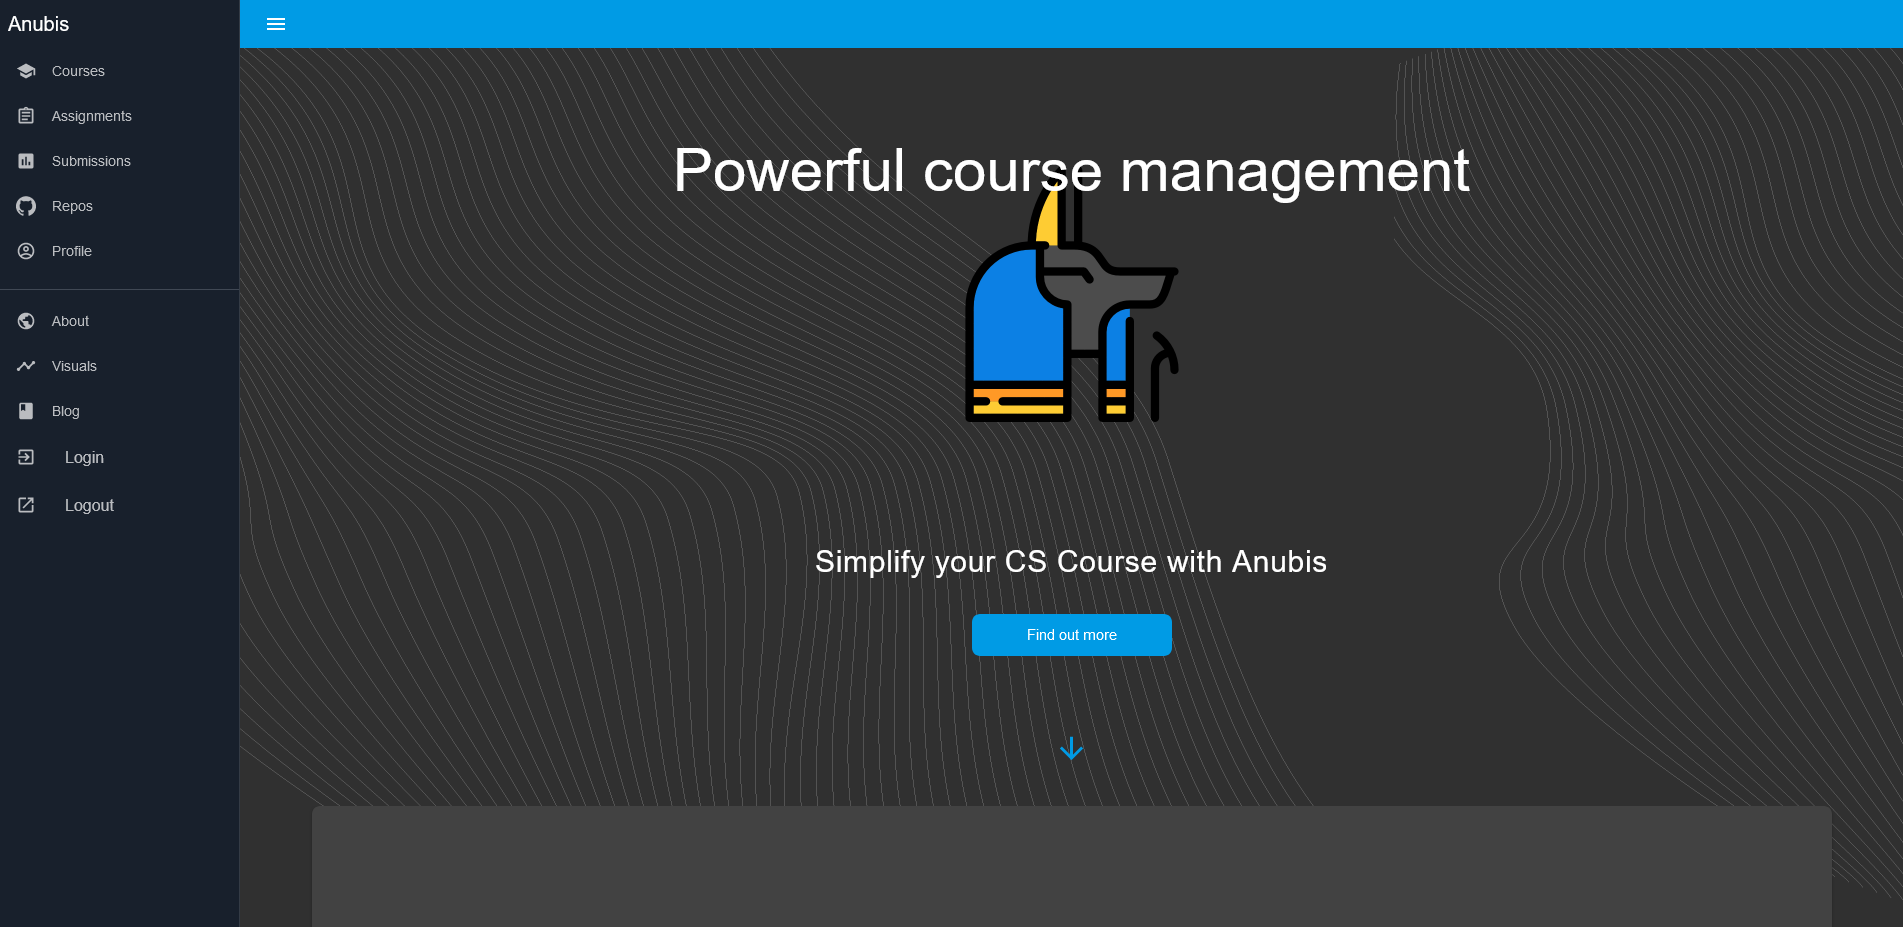
\includegraphics[width=0.75\textwidth]{figures/anubis-frontend.png}
    \caption{Anubis Web Frontend\label{fig:web-frontend}}
\end{figure}

The web static service is nothing more than a simple static http webserver.
There are no moving parts that are necessary for this service.
Only the compiled reactjs, html and css files are found in this service.
One thing of note that is not in this service are most images.
The only images that are in this web static image are the logo favicons
and some others.
The majority of images that are on the frontend (through the blog or assignment questions and whatnot)
are saved in the database and accessed through the api~\ref{sec:api}.

The frontend is designed to be a simple reflection of the backend data.
Once authenticated, users will be able to see the classes they are a part of,
current and past assignments, and all their submissions.
With few exceptions, the frontend is a near one to one translation of the API's data models.
Most pages will have a corresponding API endpoint.
The data shown on that page will be in exactly the form of the API response.


\section{Anubis Theia Proxy}\label{sec:theia-proxy}

The purpose of the the theia-proxy service it to route and forward student requests
to the appropriate Cloud IDE~\ref{ch:cloud_ides} instances.
Internals of this service are described in section~\ref{subsec:balancing-network-traffic}

\section{Reaper CronJob}\label{sec:reaper}

Many of the resources that Anubis allocates within the cluster are short lived.
The Cloud IDE, and Submission Pipeline pods are the most fluid of all.
The Cloud IDEs will be created and destroyed at the behest of students.
The Submission Pipeline pods rarely last for more than a few minutes. 
For these reasons Anubis needs a frequent recurring job that keeps resources in check.
This is where the reaper job comes in. 

It compares the resources that are suppose to be allocated according to 
the database, and the resources that are actually allocated in the cluster. 
If there are IDE or Submission Pipeline resources that are allocated that 
cannot be accounted for, or should be deleted, the reaper will schedule
them for deletion.

\subsection{Reaping IDE Resources}\label{subsec:reaping-ide-resources}

When an IDE is created by a user, there is a record of the session added to the database.
With this table of records, the reaper can pull all the IDE resources that should exist.
The reaper can then pull the IDE resources that do exist from the Kubernetes api.

Comparing these two sets there may be resources that should not exist that do, or
resources that should exist that do not.
The reaper will delete resources that should be deleted or mark sessions as ended
if the resources do not exist.

There is also a hard 6 hour limit on Anubis Cloud IDEs.
Without this limit, many students would create a Cloud IDE and just forget about it.
Obviously having these resources outstanding would be an expensive problem for Anubis to have.
The reaper handles this situation by checking for active IDEs that have reached that 6 hour limit,
and schedules the resources for deletion.

In an interesting experiment in human behavior, we can plot the cumulative duration (in minutes) of
Cloud IDEs from the final exam from CS-UY 3224's fall 2020 semester~\ref{fig:theia3}.
About 60\% of all IDE sessions reached the 6 hour limit.

\begin{figure}[ht]
    \centering
    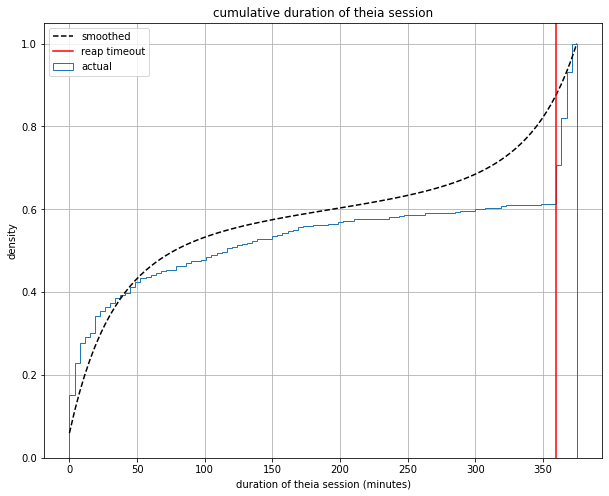
\includegraphics[width=0.5\textwidth]{figures/theia3.png}
    \caption{Cumulative Duration of a Theia Session\label{fig:theia3}}
\end{figure}

\subsection{Reaping Submission Pipeline Resources}\label{subsec:reaping-submission-pipeline-resources}

Submission Pipelines are run as Kubernetes batch jobs.
Batch jobs are not automatically removed (at least not without enabling
\href{https://kubernetes.io/docs/concepts/workloads/controllers/ttlafterfinished/}{ttl-controllers}).
Finished Submission Pipeline jobs are unnecessary resources.

For this reason, the reaper job will also schedule all finished and successful Submission Pipeline batch jobs
for deletion.
Pipeline jobs that failed for whatever reason are not deleted.
This is purposeful in design so that if there is an issue with a pipeline,
there are logs that can be examined.

\subsection{Searching and Fixing Broken Submissions}\label{subsec:reaping-fixing}

The last main responsibility of the reaper is fixing broken submissions.
Anubis is what is called an \href{https://en.wikipedia.org/wiki/Eventual_consistency}{Eventually Consistent}
system.
That means that there is a certain tolerance of short term inconsistency that is expected and
handled.
Most inconsistencies are fixed by the reaper cron.

The reaper cron searches recent submissions for common signs of breakage.
These breakages could be inconsistencies that were caused by a failed or stalled Submission Pipeline
for example.
Depending on the issue, the reaper may be able to fix or not.
For issues that cannot be fixed by the reaper, the submission is marked as broken.

Often if a student complains about some kind of inconsistency, the problem is fixed
before an Anubis admin can inspect it.
The reaper has saved countless hours for students and staff alike.

\section{RPC in Anubis}\label{sec:rpc-in-anubis}

Remote Procedural Calls are common place is many distributed systems.
Anubis relies on them quite heavily.
Many workflows in Anubis push work to RPC job queues through using the
\href{https://python-rq.org}{python-rq} library.

These calculations happen asynchronously in worker deployments on the cluster.
RPC worker pods have additional \href{https://kubernetes.io/docs/reference/access-authn-authz/rbac/}{RBAC}
permissions that the api does not have.
These permissions enable these worker instances to interface with the kubernetes api in ways
that the api cannot.
The RPC workers can create and destroy Cloud IDE~\ref{ch:cloud-ides}
and Submission Pipeline~\ref{sec:submission-pipelines} resources in the cluster.

Jobs are organized into separate queues depending on the subject of the job.
To learn more behind the reasoning for this separation, check out the
\href{Spring 2021 Midterm Retro}{https://anubis.osiris.services/blog/midterm-retro}
blog post.

\subsection{Regrade RPC}\label{subsec:regrade-rpc}

Submission Pipeline create and or regrade jobs end up in the regrade queue.
The main reason this exists as its own queue is for bulk regrades.
When running a bulk regrade on an assignment there may be a surge of thousands of
jobs enqueued into the rpc queue (one for each submission).
To avoid a bulk regrade surge draining jobs triggered by student from resources,
this exists as its own queue

\subsection{Theia RPC}\label{subsec:theia-rpc}

All jobs that have to do with the Anubis Cloud IDEs~\ref{ch:cloud-ides} end up in the theia rpc queue.
When students click the button to launch, or to stop a Cloud IDE a job is enqueued to create or destroy 
the resources on the cluster.

For the deletion of IDE resources, the stop of the session appears to be immediate.
The resources are marked as deleted in the 

\subsection{Default RPC}\label{subsec:default-rpc}

Every job that is not a submission regrade or for a Cloud IDE makes its way to the default queue.
Some of these jobs include the generation of visual data (either in raw form or image files) and
autograding results.

%    6. deployment
    \chapter{Deployment}\label{ch:deployment}

\section{Data Stores}\label{sec:data-stores}

State in Anubis is somewhat fluid.
Data is parked either in the main Mariadb~\ref{subsec:mairadb} database, or
in the redis cache~\ref{subsec:caching}.

\subsection{Mariadb}\label{subsec:mariadb}

The main data store for Anubis is a \href{https://mariadb.org/}{MariaDB}
\href{https://mariadb.com/kb/en/galera-cluster/}{galera} deployment.
More specifically the
\href{https://github.com/bitnami/charts/tree/master/bitnami/mariadb-galera}{Bitnami mariadb-galera} chart is used.

The advantage of galera is that MariaDB is multi-leader.
Any node of the MariaDB cluster can be read or written to at any time.
In a multi leader database deployment there is a certain tolerance of downed nodes before
service is degraded.
Even if nodes begin to fail, the MariaDB pods that are available can still handle
read and write operations.

All persistent storage in Anubis is parked in MariaDB.
Things like student, course and assignment information are stored here.
Temporary values like autograde results are stored in redis~\ref{subsec:redis}.

\subsection{Redis}\label{subsec:redis}

\href{https://redis.io/}{Redis} in Anubis is where temporary values are stored.
It is assumed that redis is not persistent.
What this means is that the redis deployment should be able to be reset
at any time without critical data loss.
If and when values need to be persisted, MariaDB~\ref{subsec:mariadb} is the better option.

\subsection{Caching}\label{subsec:caching}

Caching in Anubis is handled by the
\href{https://flask-caching.readthedocs.io/en/latest/index.html}{flask-caching} library.
The return values for specific functions can be temporarily stored in Redis for some
period of time.

In the Anubis API there is a great deal of caching.
Almost all view functions that query for database values will cache the results in redis
for some period of time.

Many of the computationally intensive calculation results are cached.
Take the autograde results for example.
To calculate the best submission for a student, all the
calculated submission results for that student and assignment must be pulled
out of the database and examined.
Depending on the student and assignment, this calculation could involve
examining hundreds of submissions searching for the best.
The results for these autograde calculations are then stored in the cache.

For a 3 week window around each assignment deadline the autograde results
for the assignment are periodically calculated.
The purpose of this preprocessing is to ensure that the autograde results
for recent assignments are always available in the cache.
Without this small optimization, the autograde results page in the admin
panel would just about always require 15-30 seconds to load data.

Another example of heavy caching in Anubis would be the public usage visuals.
The visuals themselves are png images that are generated from matplotlib.
To generate the png we must periodically pull out all the submission
and cloud ide session information.
Pulling this data then generating the png can take upwards of 45 seconds to a minute.
45 seconds is obviously an unacceptable amount of time to wait for an image to load
in the browser.
Anubis handles this situation by telling the API to always load the cached png image
from the cache.
The image is then periodically re-generated in the Reaper Cronjob.

Without heavy caching on things like the autograde results and visual generation
the admin panel would be quite slow.

\subsection{RPC Queues}\label{subsec:rpc-queues}

\section{Logging}\label{sec:logging}
\subsection{Filebeat}\label{subsec:filebeat}
\subsection{Elasticsearch}\label{subsec:elasticsearch}

\section{Kubernetes}\label{sec:kubernetes}
\subsection{Helm Chart}\label{subsec:helm-chart}
\subsection{Longhorn}\label{subsec:longhorn}
\subsection{Digital Ocean}\label{subsec:digital-ocean}
\subsubsection{Nodes}\label{subsubsec:digital-ocean-nodes}
\subsubsection{Networking}\label{subsubsec:digital-ocean-networking}

\section{Github}\label{sec:github}
\subsection{Github Classrooms}\label{subsec:github-classrooms}





\end{document}
